\chapter{PhD Project}

Our goal is to study sequence assembly algorithms and
various subproblems associated with them.
We already published paper about genome assembly by maximum likelihood \citep{GAML}
which opens several possibilities for further research.

In the following section we will shortly describe our assembly algorithm
and several problems which are actually open for further research.
In most cases we plan to introduce novel algorithmic ideas
and evaluate them experimentally on real and simulated datasets.

\section{Genome Assembly by Maximum Likelihood}

Our algorithm uses the following idea.
The likelihood  mentioned in \cite{Ghodsi2013} and described in Section \ref{sec:prob} 
is thought to be a good metric of the assembly quality.
Also, it can seamlessly calculate score for various types of read libraries without need
for any special algorithms and heuristics. 
Thus, our goal will be to produce the assembly with the highest possible likelihood.

The search space of this problem is huge, and consequently 
we need to resort to heuristics.
Our algorithm consists of three steps.
The first step is preprocessing, where we significantly restrict the search
space of the problem
by building de Bruijn graph and restricting our assemblies to set of walks
in this graph. Next, we use simulated annealing to find set of walks
with a high likelihood (ideally it would be maximum likelihood).
In postprocessing we look for possible
ambiguities in the assembly and split our assembly around these ambiguities.

\paragraph{Preprocessing.} In preprocessing we build de Bruijn graph from reads
using Velvet \citep{Velvet} and apply simple heuristics to this graph
 (mainly removing errors and joining vertices which can be joined ambiguously).
After preprocessing, our optimization task changes to find the set walks
in the de Bruijn graph which induce assembly with the highest likelihood.

\paragraph{Optimization by simulated annealing.}

To find a high likelihood assembly, we use an iterative
simulated annealing scheme. We start from an initial assembly $A_0$
in the assembly graph. In each iteration, we randomly choose a
\emph{move} that proposes a new assembly $A'$ similar to the current
assembly $A$. The next step depends on the likelihoods of the
two assemblies $A$ and $A'$ as follows:
\begin{itemize}
\item If $\LAP(A'|R)\ge \LAP(A|R)$, the new assembly $A'$ is accepted and
  the algorithm continues with the new assembly.
\item If $\LAP(A'|R)< \LAP(A|R)$, the new assembly $A'$ is accepted
  with probability\linebreak $e^{(\LAP(A'|R)-\LAP(A|R))/T}$; otherwise $A'$ 
  is rejected and the algorithm retains the old assembly $A$ for
  the next step.
\end{itemize}
Here, parameter $T$ is called the temperature, and it changes over time.
%In
%general, the higher the temperature, the more aggressive moves are
%permitted. We use a simple cooling schedule, where $T = T_0/\ln(i)$
%in the $i$-th iteration. The computation ends when there is no
%improvement in the likelihood for a certain number of iterations.
%We select the assembly with the highest
%$\LAP$ score as the result.

To further reduce the complexity of the assembly problem, we 
classify all contigs as either \emph{long} (more than 500bp) 
or \emph{short}
and concentrate on ordering the long contigs correctly. 
The short contigs are used to fill the gaps between the
long contigs. 
%Recall that each assembly is a set of walks in the assembly graph. 
%A contig can appear in more than one walk
%or can be present in a single walk multiple times.

\begin{figure}[t]
\centerline{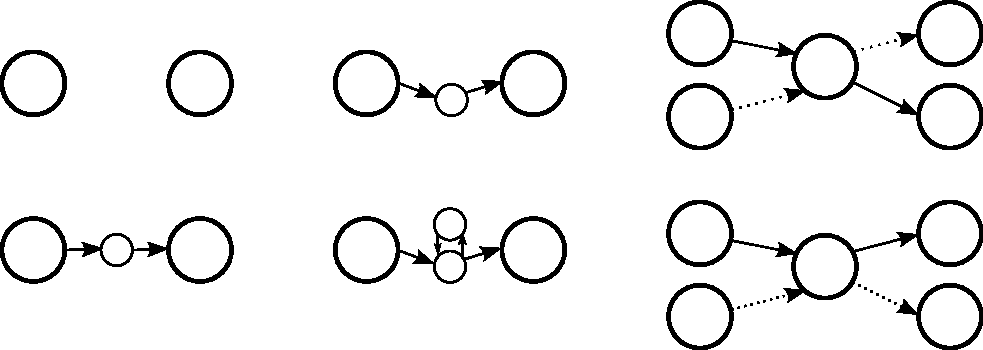
\includegraphics[width=0.8\textwidth]{../figures/p3.pdf}}
\hphantom{a}\hfill(a)\hfill\hfill(b)\hfill\hfill(c)\hfill~
\caption{{\bf Examples of proposal moves.} (a) Walk extension joining
two walks. (b) Local improvement by addition of a new loop.
(c) Repeat interchange.
\label{fig:moves}
}
\end{figure}

Proposals of new assemblies are created from the current assembly
using the following moves (and more others):
\begin{itemize}
\item \emph{Walk extension.} (Fig.\ref{fig:moves}a)
  We try to join the two walks into one by adding a small walk between them.
%  We start from one end of an existing walk and randomly walk
%  through the graph, at every step uniformly choosing one of the
%  edges outgoing from the current node.
%  Each time
%  we encounter the end of another walk, the two walks are considered for
%  joining. We randomly (uniformly) decide whether we join the walks,
%  end the current walk without joining, or continue walking.
\item \emph{Local improvement.} (Fig.\ref{fig:moves}b)
  We optimize the
  part of some walk connecting two long contigs $s$ and $t$.
%  We first
%  sample multiple random walks starting from contig $s$. In each walk,
%  we only consider nodes from which contig $t$ is reachable. Then we
%  evaluate these random walks and choose the one that increases the
%  likelihood the most.
%  If the gap between contigs $s$ and $t$ is too big, we instead 
%  use a greedy strategy where in each step we explore  
%  multiple random extensions of the walk of length 
%  around 200bp and pick the one with the highest
%  score.
%\item \emph{Repeat optimization.} We optimize the copy number of 
%  short tandem repeats. We do this by removing or adding a loop
%  to some walk. We precompute the list of all short loops (up to five nodes) in the graph
%  and use it for adding loops.
%\item \emph{Joining with advice.} We join two walks that are spanned by long 
%  reads or paired reads with long inserts. We fist select a starting walk, align
%  all reads to the starting walk and randomly choose a read which has 
%  the other end
%  outside the current walk. Then we find to which node this other end
%  belongs to and join appropriate walks.
%  If possible, we fill the gap between the two walks using the
%  same procedure as in the local improvement move. Otherwise we introduce
%  a gap filled with Ns.
\item \emph{Disconnecting.} We remove a path through short contigs 
  connecting two long contigs in the same walk, resulting in two
  shorter walks.
\item \emph{Repeat interchange.} (Fig.\ref{fig:moves}c) 
  If a long contig has several incoming and outgoing walks
  we try to swap pairing of incoming and outgoing edges.
  %If a long
  %contig has several incoming and outgoing walks, we optimize the
  %pairing of incoming and outgoing edges. In particular, we evaluate
  %all moves that exchange parts of two walks through this contig. If
  %one of these changes improves the score, we accept it and repeat
  %this step, until the score cannot be improved at this contig.
\end{itemize}

At the beginning of each annealing step, the type of the move is
chosen randomly; each type of move has its own probability. We also
choose randomly the contig at which we attempt to apply the move. 

%Note that some moves (e.g. local improvement) are very general, while
%other moves (e.g. joining with advice) are targeted at specific
%types of data. This does not contradict a general nature of our
%framework; it is possible to add new moves as new types of data
%emerge, leading to improvement when using specific data sets, while
%not affecting the performance when such data is 
%unavailable.

\paragraph{Postprocessing.}
The assembly obtained by the simulated annealing may contain walks
with no evidence for a particular configuration of incoming and
outgoing edges in the assembly graph. This happens for example if a
repeat is longer than the span of the longest paired read. In this
case, there would be several versions of the assembly with the same or
very similar likelihood score. 
In the postprocessing step, we therefore apply the repeat
interchange move at every possible location of the assembly. If the
likelihood change resulting from such a move is negligible, 
we break the corresponding walks into shorter contigs
to avoid assembly errors. 

\paragraph{Fast likelihood evaluation}
In each step of the simulated annealing we need to calculate
the assembly likelihood. This step involves
alignment of a large number of reads to the assembly.
However, only a small part of the assembly is changed in each
annealing step, which we can use to significantly reduce the running time.

Our main ideas are following:
\begin{itemize}
\item {\bf Aligning reads only to changed portions of the assembly.}
Since only a small portion of the assembly is changed in each step, 
we can cache most alignments from the previous iterations and only 
align reads to the changed sequence regions.
\item {\bf Reducing the number of reads which need to be aligned.}
We use a simple prefiltering step to
find the reads which are likely to align to the target sequence. 
We look for reads which 
contain some $k$-mer (usually $k=13$) from the target sequence.
For this we need to maintain an index of all $k$-mer in reads, which is
quite memory consuming and we are looking into better data structures for this kind
of problem.
\end{itemize}

\paragraph{Experimental results}
We developed a prototype for described algorithm, called GAML and
demonstrated that it can obtain high quality assemblies
for small genomes (up to ten million bases). The details
of the experiments can be found in \citet{GAML}.

\section{Improvements of GAML}

We want to improve GAML to be able to assemble larger genomes.
The room for improvement is mainly in the following areas:

\paragraph{Better moves.}
The current moves are too general and need many tries to
find an assembly with higher likelihood. We want to develop
moves which will also rely on some information from reads
and thus be able to be more precise and improve
assembly more rapidly. Also our moves
do not exploit any structure in the de Bruijn graph (except for the connectivity)
and this could lead to even better moves.

\paragraph{Marking some moves as most likely good and applying moves in batches.}
If we are able to use some information from reads and de Bruijn graph
then we should be able to mark some moves as "with high probability will increase
assembly likelihood". Then we can make few of this moves in one
batch and evaluate assembly likelihood after doing all of them
and not after each one.

\paragraph{More efficient evaluation of assembly likelihood.}
This includes reducing amount of calculation during evaluation.
Now, we still calculate likelihood for each read (our optimization
mainly reduces time spent on aligning reads). This can
be improved by using smarter memoization patterns.
Furthermore, we can reduce memory requirements
of read indexing, as discussed in next section.

\section{Efficient Indexing of Read Libraries}

We need to keep index of all reads to be
able to quickly evaluate assembly likelihood in our assembler.
Our current implementation of index uses hash map, which
has big memory requirements.
Our goal is to develop a data structure for indexing
reads which has smaller memory footprint.
This data structure should be able to index reads
and answer queries of type: which reads contain
a given $k$-mer (with an upper bound on $k$ specified at the time
of constructing the data structure). Optionally,
it can support alignment of reads to given sequence.

There has been several data structures proposes for
indexing reads, e.g. \cite{GKArrays} and \cite{CGKArrays}.
None of these data structures exploit the fact
that reads come from the same underlying sequence.

In our proposed approach we will
first find some approximation of the underlying sequence.
This task is similar to the sequence assembly, but our goal
is not to reconstruct the underlying sequence exactly, but achieving a compact
representation of reads. Thus, we can collapse repeats, and do other things
which are inadvisable during sequence assembly.
This representation can be either one string or a graph similar to
de Bruijn graph. Then, each read can be represented
as a part of the representation plus some small edits (since
reads can contain errors).

The querying will be done by search for $k$-mers in the underlying
sequence and then finding relevant reads connected to the resulting
parts of the underlying sequence. We also believe
that we can extend the query for finding alignments of reads to a given sequence.

\section{Algorithms for Reads with High Number of Errors}

The most recent technologies like PacBio \citep{PacbioToCA} and Oxford
Nanopore \citep{oxford} produce reads with high number of errors
($15\%$ for PacBio \citep{PacbioToCA}, $35\%$ for Oxford Nanopore \citep{oxford}).
Current tools are not designed to work with such erroneous reads.

There are several possible directions for further research:

\paragraph{Mapping reads to the genome.} The state of art tool
for this task is BLASR \citep{BLASR}. We believe
that it can be further improved by ideas for aligning erroneous reads
mentioned in \citet{myers2014efficient}. 
Myers uses sorting and merging instead of indexing with hash maps,
which is in practice faster due to better cache locality.
He also cleverly cuts search space in dynamic programming for finding mapping
with smallest edit distance.
We can also use ideas from \cite{MHAP}, which are mainly filtering
possible matches by using Jaccard similarity of $k$-mers in relevant areas
and using min-hashing.

\paragraph{Self correction of reads.}
Currently, a typical procedure for assembling erroneous reads
starts with aligning of reads to each other, then using this alignments
to correct given reads and then running overlap-layout-consensus assembler
as was done in \cite{MHAP}.
The most time consuming step is the alignment of reads.
We believe that if we have big coverage (around $40$ times and more) then
we do not need precise alignment of reads and that we can
correct reads using much faster heuristics. For example
we can mark some areas in reads as "probably correct" if we can
find support for them in other reads. Then we can
use this sequencing for correcting reads.

\paragraph{Mapping contigs to long reads without basecalling.}
Reading DNA is fuzzy process and most of the DNA sequencing
methods rely on probabilistic models to produce final DNA
from raw data. The process of producing final DNA is called basecalling.
We think that we could produces better alignments when
we use raw data instead of DNA sequences, since they can give
us probability distributions for possible errors. 

\label{LastPage}

